%#######################################################################################
%############################		CABECERA		####################################
%#######################################################################################
\documentclass[a4,12pt,onecolum]{article}
\usepackage[utf8]{inputenc}
\usepackage[spanish]{babel} 		% para que divida bien las silabas en final de linea
\usepackage[margin=3cm]{geometry}	% para poner los margenes bonitos
\usepackage{fancyhdr}
\usepackage{graphicx} 				% meter figuras gráficas
\graphicspath{{fotos/}}
\usepackage{import}
\usepackage{color} 					% para introducir colores en el documento
\usepackage{verbatim}
\usepackage{subfigure}
\usepackage{listings}
\usepackage{cite}
%\bibliographystyle{alpha}
\usepackage{graphicx}
\usepackage{fancyhdr}
\usepackage{subfigure}
\usepackage{listings, courier}
\usepackage{amssymb, amsmath, amsbsy}
\usepackage{float}
\usepackage[colorinlistoftodos]{todonotes}
\usepackage{cite}
\PassOptionsToPackage{hyphens}{url}\usepackage{hyperref}
\usepackage{url, hyperref}
\usepackage[nottoc]{tocbibind}
\usepackage{titlesec}
\usepackage{fancyvrb}
\setlength{\headheight}{20pt}


% FIGURAS [htbp] significa que el orden para que LaTeX trate de incrustar la imagen es: primero que lo intente aquí (h), luego en la parte de arriba (t), a continuación, en la parte de abajo (b), y por último, en la parte de arriba de la siguiente página (p). Puedes reordenar estas letras para seleccionar el orden que prefieras. Eso sí, muchas veces LaTeX hace lo que quiere. Pero si pones [htbp], indicas a LaTeX que ponga la imagen exactamente ahí. Para usar [htbp] tienes que cargar el paquete {float}.


%\usepackage{times} 						% tipo de letra periodico
%\renewcommand{\familydefault}{\sfdefault}	% tipo de letra Arial

% este bloque es para definir el estilo del texto C++
\lstset{language=C++,
  inputencoding=latin1,	% permite las tildes en el código
  backgroundcolor=\color[gray]{0.9},% color del fondo
  frame=single,		% dibuja un borde
  columns=flexible,	% el tamaño de letra se ajusta al ancho
  extendedchars=false,
  aboveskip=1eM,
  basicstyle=\ttfamily,
  keywordstyle=\color{blue}\ttfamily,
  stringstyle=\color{red}\ttfamily,
  commentstyle=\color{green}\ttfamily,
  morecomment=[l][\color{magenta}]{\#}
}

\hypersetup{
    bookmarks=true,         % show bookmarks bar?
    unicode=false,          % non-Latin characters IN Acrobat’s bookmarks
    pdftoolbar=true,        % show Acrobat’s toolbar?
    pdfmenubar=true,        % show Acrobat’s menu?
    pdffitwindow=false,     % window fit to page when opened
    pdfstartview={FitH},    % fits the width of the page to the window
    pdftitle={My title},    % title
    pdfauthor={Author},     % author
    pdfsubject={Subject},   % subject of the document
    pdfcreator={Creator},   % creator of the document
    pdfproducer={Producer}, % producer of the document
    pdfkeywords={keyword1} {key2} {key3}, % list of keywords
    pdfnewwindow=true,      % links IN new PDF window
    colorlinks=true,        % false: boxed links; true: colored links
    linkcolor=black,          % color of internal links (change box color with linkbordercolor)
    citecolor=blue,        % color of links to bibliography
    filecolor=magenta,      % color of file links
    urlcolor=blue           % color of external links
}

%\usepackage[hidelinks]{hyperref}% para anadir enlace dentro del documento, tiene que ser la ultima declaracion porque sino puede fallar

\title{Seguridad}
\date{\today}

%---------------------- ENCABEZADO Y PIE DE PÁGINA

\pagestyle{fancy}

\lhead{Seguridad}
\rhead{\leftmark}
\cfoot{\thepage}

\renewcommand{\headrulewidth}{0.4pt} % grosor de la línea de la cabecera
\renewcommand{\footrulewidth}{0.4pt} % grosor de la línea del pie


\setcounter{secnumdepth}{4}
\titleformat{\paragraph}
{\normalfont\normalsize\bfseries}{\theparagraph}{1em}{}
\titlespacing*{\paragraph}
{0pt}{3.25ex plus 1ex minus .2ex}{1.5ex plus .2ex}
%#######################################################################################
%##############################			CUERPO			################################
%#######################################################################################
\begin{document}

%################## PORTADA

\begin{titlepage}

\newcommand{\HRule}{\rule{\linewidth}{0.5mm}} % Defines a new command for the horizontal lines, change thickness here

\center % Center everything on the page

\textsc{\LARGE Universidad de Murcia}\\[0.8cm]
\textsc{\Large Grado en Ingeniería Informática}\\[0.5cm]
\textsc{\large 4º curso}\\[0.4cm]
\textsc{\large Grupo 6}\\[0.4cm]
\textsc{\large Curso 2016/2017 - Junio}\\[0.4cm]

\HRule \\[0.6cm]
{ \huge \bfseries Seguridad}\\[0.3cm]
\HRule \\[0.5cm]
{ \Large \bfseries Práctica final}\\[0.3cm]
\HRule \\[1.0cm]

%################## AUTORES

\begin{minipage}{0.4\textwidth}
\begin{flushleft} \large
Alumnos:\\
Cristian Roche Borja \\
\small{DNI: 76581531H}	\\
\large{Alicia Ruiz Tovar} \\
\small{DNI: 48693813F}
\end{flushleft}
\end{minipage}
~
\begin{minipage}{0.4\textwidth}
\begin{flushright} \large
Docentes: \\
Alberto Huertas Celdrán
Gabriel López Millán
Gregorio Martínez Pérez
\end{flushright}
\end{minipage}\\[1cm]

%################## LOGO

\centering

\includegraphics[width=0.5\textwidth]{./portada/logoum.png}\\[0.8cm] % Include a department/university logo - this will require the graphicx package

\end{titlepage}

%################## PAGINA EN BLANCO

\thispagestyle{empty}
\textcolor[rgb]{1.00,1.00,1.00}{palabra} % Pinta "palabra" de blanco
\newpage

\setcounter{page}{3}

%##################	TABLA DE CONTENIDOS

\newpage
\tableofcontents 		% indice
\rhead[\thepage]{Índice}
\newpage

%##################	CUERPO DEL DOCUMENTO

%################## INTRODUCCIÓN

%\section{Introducción}
%\rhead[\thepage]{\thesection. Introducción}

% #######################   OAUTH   ##################################

\clearpage
\section{Oauth}
\rhead[\thepage]{\thesection. Oauth}

\subsection{Introducción}
Open Authorization(Oauth) es un mecanismo un mecanismo de autorización, está estandarizado y es abierto, es decir, disponible públicamente para su uso. El protocolo que implementa Oauth se basa en la \emph{autorización delegada}, se hace uso de una tercera entidad para autenticar al usuario, sin embargo, esta es la utilidad más básica, una vez autenticado a un usuario, se pueden solicitar su información asociada.

Desde el punto de vista del usuario final, este sistema supone una gran ventaja, no necesita de múltiples credenciales en cada uno de los sitios web que frecuenta, basta con disponer de una cuenta de usuario válida en un servidor de autenticación, es el caso de Google, Facebook, etc... grandes empresas que ofrecen este servicio a sus usuarios.

Desde el punto de vista de una mediana empresa, resulta muy sencillo beneficiarse de este mecanismo llegando a acuerdos con empresas de autenticación, como las ya mencionadas. La inclusión en los servicios web es muy sencilla y basta con poner un botón opcional en la página que solicita las credenciales de acceso. El usuario final demostrará su identidad e incluso puede permitir el acceso diferentes apartados(scopes) de su información personal, que está siendo gestionada actualmente por Google, Facebook...

% #######################   ADAPTACIÓN A LA TOPOLOGÍA   ##################################

\subsection{Adaptación a la topología}
En nuestro grupo de prácticas, trabajamos dando servicio a un bufete de abogados, cubriendo las necesidades de los trabajadores y de los clientes del bufete. Consideremos que Oauth puede facilitar en gran medida las gestiones online de los clientes, permitiendo la compartición de sus datos con diferentes empresas colaboradoras. No supone una violación de la privacidad del cliente, ya que será este en cada momento quien decida que empresas pueden acceder a su información.

Para que Oauth tenga una apliación real en nuestra topología, es necesario incluír en la escena a una segunda empresa colaboradora, como trabajamos con abogados, es interesante la inclusión de una notaría \texttt{"Notaría Arrigaga Asociados"}. Como trabajamos con un bufete con un buen número de abogados, disponemos de una infraestructura informática  importante, la información de nuestros clientes ya está almacenada en nuestros servidores, la dirección ha decidido que el bufete implantará el servicio de autenticación con Oauth. Cualquier empresa colaboradora que esté interesada en hacer uso de nuestro servicio tendrá que firmar un acuerdo, en el que se incluye las garantías de confidencialidad y los aspectos económicos.

En el momento de la implantación, solo se ha llegado a un acuerdo con la notaría anteriormente mencionada, asumiendo cada actor los siguientes roles:
\begin{itemize}
\item \texttt{Bufete de abogados:} Será el encargado de la identificación(\emph{IDP Server}), autorización(\emph{Authorization Server}) y de servir los recursos(\emph{Resource Server}).
\item \texttt{Notaría:} Actuará como cliente (\emph{Client}).
\item \texttt{Usurio final:} Será quién hace uso del servicio mediante su navegador web y quien facilite el acceso a sus recursos(\emph{ResourceOwner}). 
\end{itemize}

En esta práctica la implementación de Oauth no solo se limitará a la autenticación de los clientes del bufete, sino que también se utilizará para facilitar parte de la información personal de los mismos, facilitando las gestiones.

% #######################   IMPLEMENTACIÓN   ##################################

\subsection{Implementación}
Utilizaremos una implementación basada en el esquema \emph{implicit} como se muestra en la figura \ref{fig:oauth1}. Esta modalidad tiene como característica principal, que es el navegador del propietario de los recursos (Resource Owner) el medio utilizado para interactuar con las diferentes entidades. Modificaremos ligeramente el esquema separando la identificación y la autenticación en dos servidores independientes.

Una vez que el \emph{User agent} haya realizado todas las peticiones previas, el \emph{Client}, en en este caso corresponde con la \emph{Notaría}, podrá realizar consultas de la información del \emph{Resource owner} de forma directa en el \emph{Client resource}, este permiso tendrá una duración de 30 segundos, expirado ese periodo, el permiso caducará. Aunque la duración de dicho permiso pueda parecer corta, el fin de esta implementación es que la Notaría pueda consultar casi de forma instantánea los datos del usuario, para rellenar  un formulario con su información personal, obtener algún documento, etc... \\

\begin{figure}[htbp]
\centering
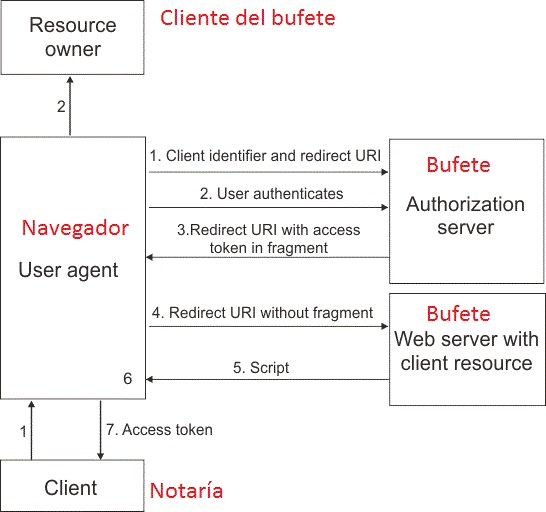
\includegraphics[width=0.8\textwidth]{./images/oauth/implicit.jpg}
\caption{Esquema implicit.}
\label{fig:oauth1}
\end{figure}

Para la realización de esta práctica, hemos implementado los servicios con Java Rest, que presenta las siguientes ventajas:
\begin{enumerate}
\item Alto rendimiento, soportando un gran número de peticiones simultáneas.
\item Claridad en el código. Se ve de forma muy clara el tipo de función implementada y el resultado que genera.
\item Permite la inclusión y lectura de cabeceras HTTP de forma muy clara y en una sola línea de código.
\item Uso dinámico de las URLs, pudiendo usarlas para recibir parámetros que forman parte de la propia URL. (http://www.notaria.es/{userID}/{userPhone}/)
\item Dispone de un amplio soporte y documentación para la resolución de problemas.
\item La librería de Oauth esta implementada también en Java Rest, por lo que se hace más sencilla la adaptación. \\
\end{enumerate}

A la hora de resolver las dependencias con otras librerías, hemos optado por el uso de \emph{Maven}, que tiene las siguientes ventajas:
\begin{enumerate}
\item Soportado de forma nativa en Eclipse.
\item Fácil conversión de un proyecto tradicional a uno maven.
\item Amplio soporte y documentación de uso.
\item No es necesario descargar las librerías, solo se incluyen las referencias y se descargan automáticamente.
\item Basándonos en el punto anterior, el tamaño del proyecto final es muy pequeño.
\item Maven dispone de la librería de Oauth en su repositorio.
\end{enumerate}

% #######################   IMPLEMENTACIÓN   ##################################

\subsubsection{URLs y Servidores}
A continuación, se muestra una lista con los diferentes servidores que hemos implementado, así como las URLs de las que dispone cada uno. Así se podrá entender de forma más clara el funcionamiento de nuestro esquema.

\begin{itemize}
\item \texttt{ServidorWeb Notaría(Client)}
	\begin{itemize}
		\item \emph{/Seguridad\_NotariaWeb/rest/Index	GET} \\
		Página de inicio de la Notaría, en la que se puede visualizar el índice de contenidos.
		
		\item \emph{/Seguridad\_NotariaWeb/rest/Formulario	GET} \\
		Muestra un mensaje indicando que el formulario al que se ha accedido necesita consultar datos 					personales del usuario, después de 5 segundos realiza una redirección. Si la Notaría no se encontraba 			registrada, realiza el registro antes de redirigir.
		
		\item \emph{/Seguridad\_NotariaWeb/rest/Resultado	GET} \\
		Se llama cuando el usuario ya ha obtenido el \emph{AccessToken} del servidor de autorización. Cuando 			recibe el \emph{AccessToken} realiza las consultas al servidor de recursos. Como resultado, se muestra 			un formulario al usuario autocompletado con sus datos personales.
	\end{itemize}
	
\item \texttt{Servidor Identificación(IDP)}
	\begin{itemize}
		\item \emph{/Seguridad\_IDP/rest/OauthRegistro	POST} \\
		Recibe las peticiones de registro, registra al \emph{Client} y envía la respuesta.
		
		\item \emph{/Seguridad\_IDP/rest/Identifier	GET} \\
		Muestra una página web en la que el usuario debe introducir la imagen de su huella digital y su DNI/			Contraseña. Al pulsar enviar, se realiza un POST a la misma URL.
		
		\item \emph{/Seguridad\_IDP/rest/Identifier	POST} \\
		Recibe la información de identificación del usuario, valida por niveles cada uno de los datos, la 				detección de un dato no válido implica no comprobar los siguientes. En primer lugar el DNI/Contraseña, 			ya que es el menos costoso desde el punto de vista computacional.
		Si se superan todos los niveles de identificación, se genera una \emph{Cookie} para el cliente.
		
		\item \emph{/Seguridad\_IDP/rest/Identifier/redirect	POST} \\
		Transforma la petición POST del cliente, que en este momento contiene la imagen de la huella y el 				usuario y contraseña, en una petición GET dirigida al servidor de autorización.
		
		\item \emph{/Seguridad\_IDP/rest/CheckAuthCookie	POST} \\		
		Esta página es invocada por el servidor de autorización para validar la \emph{Cookie} que el 					\emph{Client} le ha presentado. Recibe la \emph{Cookie} en formato Json y devuelve el \emph{ID} del 			usuario asociado a esa \emph{Cookie}, en el caso de que no sea válida, mostrará un error 401 					\emph{Unauthorized}.		
		
		\item \emph{/Seguridad\_IDP/rest/Error	GET} \\
		Página de error mostrada para indicar al usuario el fallo de alguno de los pasos.
	\end{itemize}
	
\item \texttt{Servidor Autorización(Authorize)}
	\begin{itemize}
		\item \emph{/Seguridad\_Authorize/rest/Authorize	GET} \\
		Recibe la \emph{Cookie} y los datos de identificación del \emph{Client}. En primer lugar, se verifica 			que los datos del \emph{Client} sean válidos, posteriormente se valida la \emph{Cookie} presentada 				(Esta validación se realiza lanzando una consulta al IDP {/Seguridad\_IDP/rest/CheckAuthCookie}). 				Si toda la información es correcta, se genera un \emph{AccessToken} y se redirecciona.
		
		\item \emph{/Seguridad\_Authorize/rest/CheckAccessToken	POST} \\
		Esta página es invocada por el servidor de recursos para validar el \emph{AccessToken} que el 					\emph{Client} le ha presentado. Recibe el \emph{AccessToken} en formato Json y devuelve el \emph{ID} 			del	usuario asociado a ese \emph{AccessToken}, en el caso de que no sea válido, mostrará un error 401 			\emph{Unauthorized}.
	\end{itemize}
	
\item \texttt{Servidor Recursos(Resource)}
	\begin{itemize}
		\item \emph{/Seguridad\_ResourceServer/rest/DNI	GET} \\
		Consulta al servidor de autorización la validez del \emph{AccessToken} presentado, en esta consulta 			recibe el ID del usuario asociado. Devuelve el número de DNI en formato Json.
		
		\item \emph{/Seguridad\_ResourceServer/rest/Name	GET} \\
		Consulta al servidor de autorización la validez del \emph{AccessToken} presentado, en esta consulta 			recibe el ID del usuario asociado. Devuelve el nombre en formato Json.
		
		\item \emph{/Seguridad\_ResourceServer/rest/Surname	GET} \\
		Consulta al servidor de autorización la validez del \emph{AccessToken} presentado, en esta consulta 			recibe el ID del usuario asociado. Devuelve el apellido de DNI en formato Json.
		
		\item \emph{/Seguridad\_ResourceServer/rest/Phone	GET} \\
		Consulta al servidor de autorización la validez del \emph{AccessToken} presentado, en esta consulta 			recibe el ID del usuario asociado. Devuelve el número de teléfono en formato Json.
		
		\item \emph{/Seguridad\_ResourceServer/rest/Address	GET} \\
		Consulta al servidor de autorización la validez del \emph{AccessToken} presentado, en esta consulta 			recibe el ID del usuario asociado. Devuelve la dirección en formato Json.
		
		\item \emph{/Seguridad\_ResourceServer/rest/Email	GET} \\
		Consulta al servidor de autorización la validez del \emph{AccessToken} presentado, en esta consulta 			recibe el ID del usuario asociado. Devuelve el email en formato Json.
		
		\item \emph{/Seguridad\_ResourceServer/rest/BirthDate	GET} \\
		Consulta al servidor de autorización la validez del \emph{AccessToken} presentado, en esta consulta 			recibe el ID del usuario asociado. Devuelve la fecha de nacimiento en formato Json.
	\end{itemize}
\end{itemize}

% #######################   SECUENCIA DE FUNCIONAMIENTO  INTERNO  ##################################

\subsubsection{Secuencia de Funcionamiento Interno}
La imagen \ref{fig:oauth2} muestra un diagrama de secuencia, en este diagrama se muestra gráficamente todos los mensajes enviados y recibidos desde el \emph{User Agent} y el \emph{Client}. Por simplificar el diagrama, solo se muestra la obtención del DNI, en la resolución práctica se realizan consultas de cada uno de los datos del usuario: nombre, fecha de nacimiento, DNI, apellido, dirección, email, fecha de nacimiento y número de teléfono.

\begin{enumerate}
	\item El usuario accede con su navegador a la página web principal de la Notaría.
	
	\item El usuario intenta acceder al formulario de solicitud de hipoteca, este formulario precisa de la 			autenticación del usuario y su información personal. Como el usuario ya es miembro del bufete de abogados 		(empresa colaboradora), se delega en ellos la autenticación y la obtención de recursos. Por tanto, 				redirigimos al usuario	\emph{Redirect.html}.
	
	\item La primera parada es el servidor de identificación, este devolverá al cliente una página web con un 		formulario de indentificación \emph{Identifier.html}. El usuario completará la información requerida y 			pulsará en el botón \emph{Enviar}.
	
	\item Se recibe la información de identificación en el servidor IDP, se valida, se genera la 					\emph{CookiePass} y se responde con una redirección \emph{Redirect.html}.
	
	\item Esta última redirección simplemente convierte el mensaje POST que aún contiene la huella y el DNI y 		contraseña en un mensaje GET, redirigiendo nuevamente al servidor de autorización \emph{Authorize.html}.
	
	\item El servidor de autorización recibe la \emph{CookiePass}, verifica que la petición sea lícita, valida 		la \emph{CookiePass}(consultando al IDP si es válida), genera un \emph{AccessToken} y realiza una 				redirección a la web de la Notaría \emph{Resultado.html}. 
	
	\item Llegados a este punto, la Notaría ya tiene el código con el que puede realizar las consultas en el 		servidor de recursos, en cada petición presentará el \emph{AccessToken}. Por ejemplo, \emph{dni.html} para 		obtener el DNI.
	
	\item El servidor de recursos solo recibe el \emph{AccessToken}, no necesita recibir más información, 			porque al consultar al servidor de autorización si es válido, este puede contestar o bien, diciendo que no 		es un código válido \emph{401 Unauthorized} o, con el ID del usuario al que pertenece ese 						\emph{AccessToken} en formato Json. Teniendo el ID del usuario, el servidor de recursos consulta en su base 	de datos y responde con los datos solicitados en formato Json.
	
	\item La Notaría está programada de tal forma que realizará tantas peticiones como sean necesarias para 		obtener la información requerida por el formulario. Como resultado, se mostrará el formulario al usuario 		final totalmente autocompletado \emph{Resultado.html(Autocompleted)}.
	
	
\end{enumerate}

\begin{figure}[htbp]
\centering
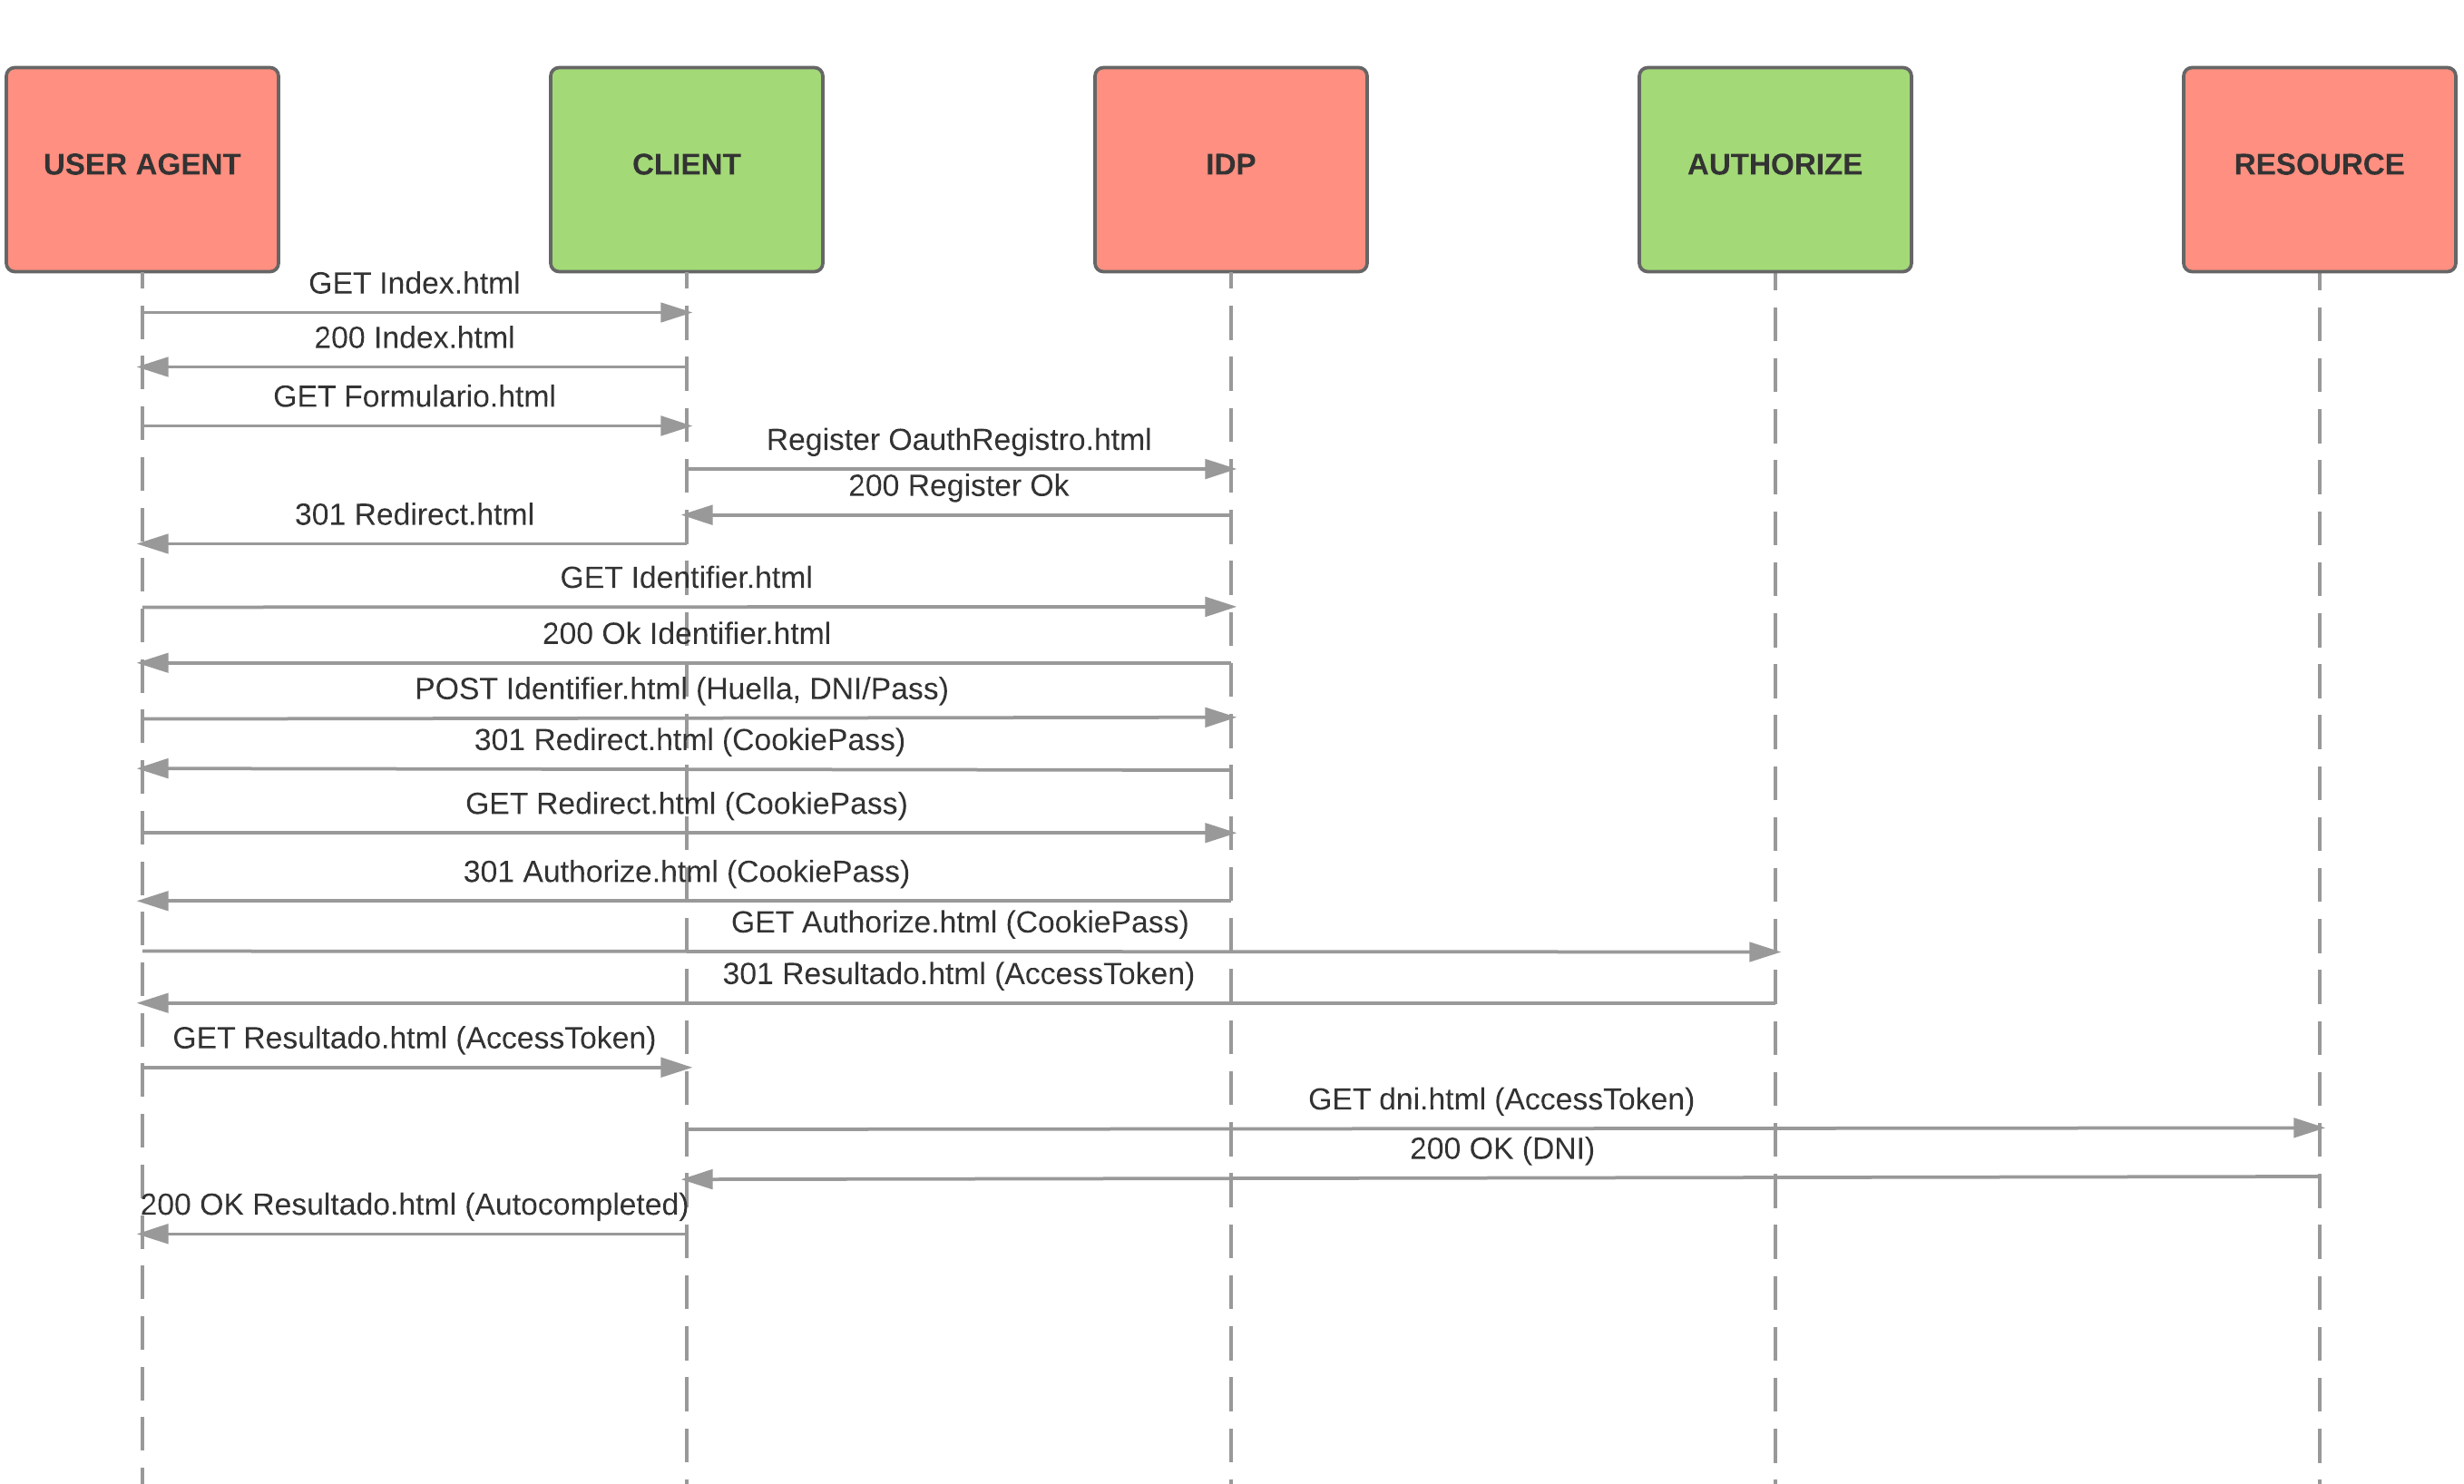
\includegraphics[width=1.1\textwidth]{./images/oauth/diagrama_flujo_useragent.png}
\caption{Diagrama User Agent.}
\label{fig:oauth2}
\end{figure}

En la figura \ref{fig:oauth3} se muestra el diagrama de secuencia de la obtención del \emph{AccessToken}, el \emph{User Agent} lanza la petición con la \emph{Cookie} al servidor de autorización, este comprueba la validez de la misma consultando al servidor de identificación (quien la generó), este responderá indicando si es válida o no, en caso de serlo, el servidor de autorización genera un \emph{AccessToken} y se lo entrega al \emph{User Agent}. \\

\begin{figure}[htbp]
\centering
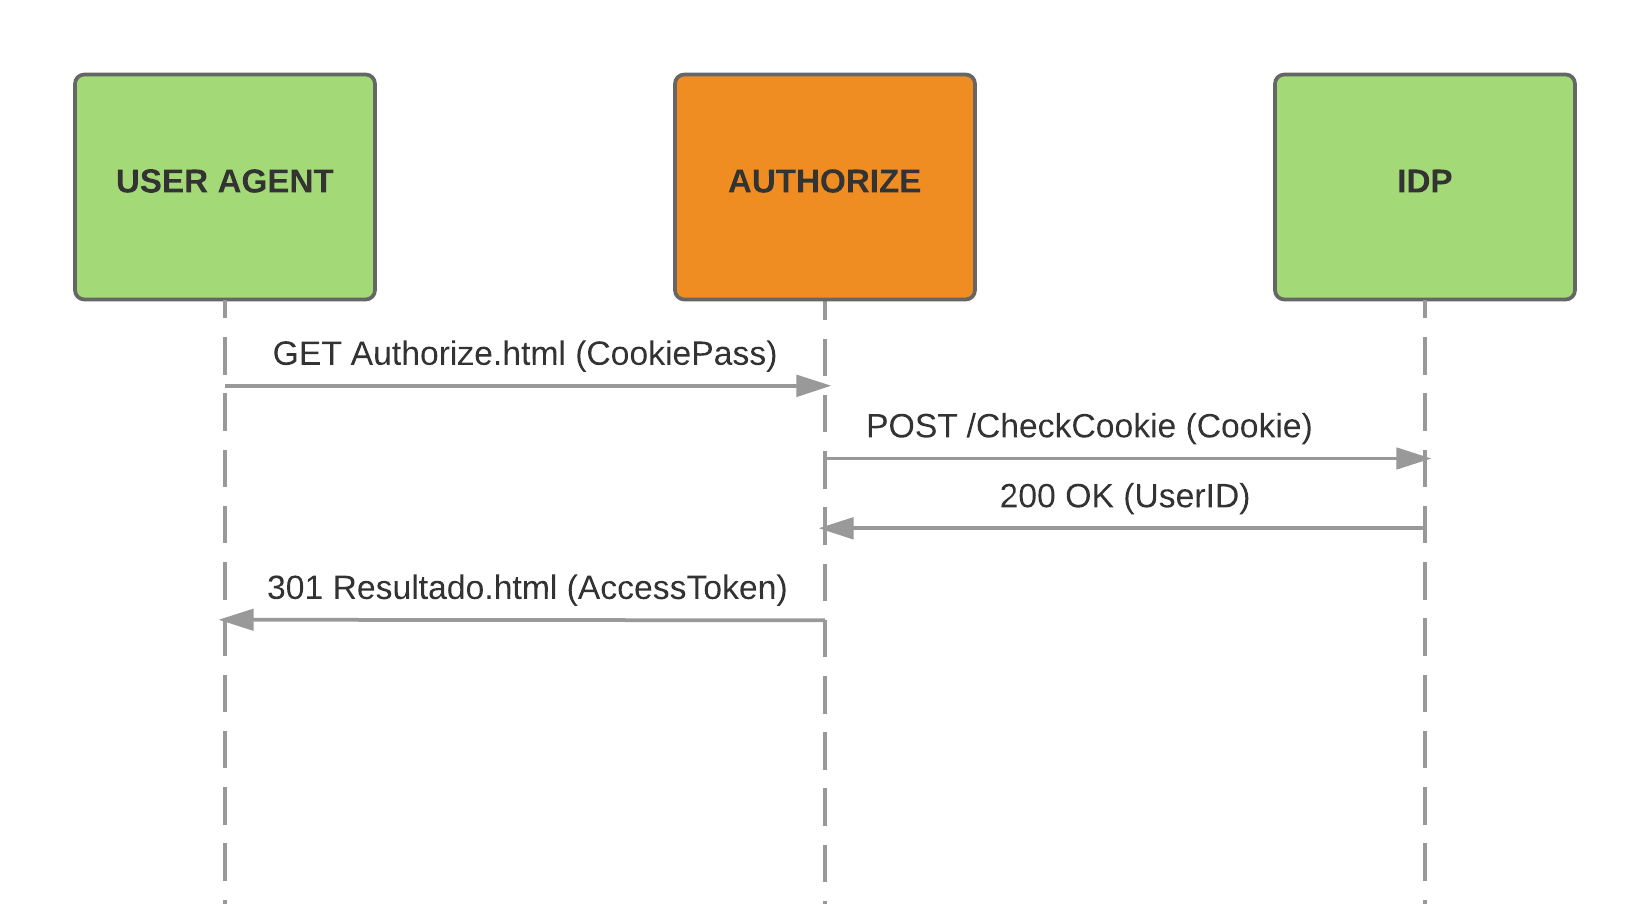
\includegraphics[width=1.1\textwidth]{./images/oauth/diagrama_secuencia_getToken.png}
\caption{Diagrama obtener AccessToken.}
\label{fig:oauth3}
\end{figure}


En la figura \ref{fig:oauth4} se muestra el diagrama de secuencia de la obtención de un recurso. El \emph{Client} manda la solicitud al servidor de recursos adjuntando el \emph{AccessToken}, el servidor de recursos lo valida consultando al servidor de autorización (quien lo generó), si es válido, el servidor de autorización responde con el ID del usuario asociado. Finalmente, el servidor de recursos entrega el recurso al \emph{Client}.	\\

\begin{figure}[htbp]
\centering
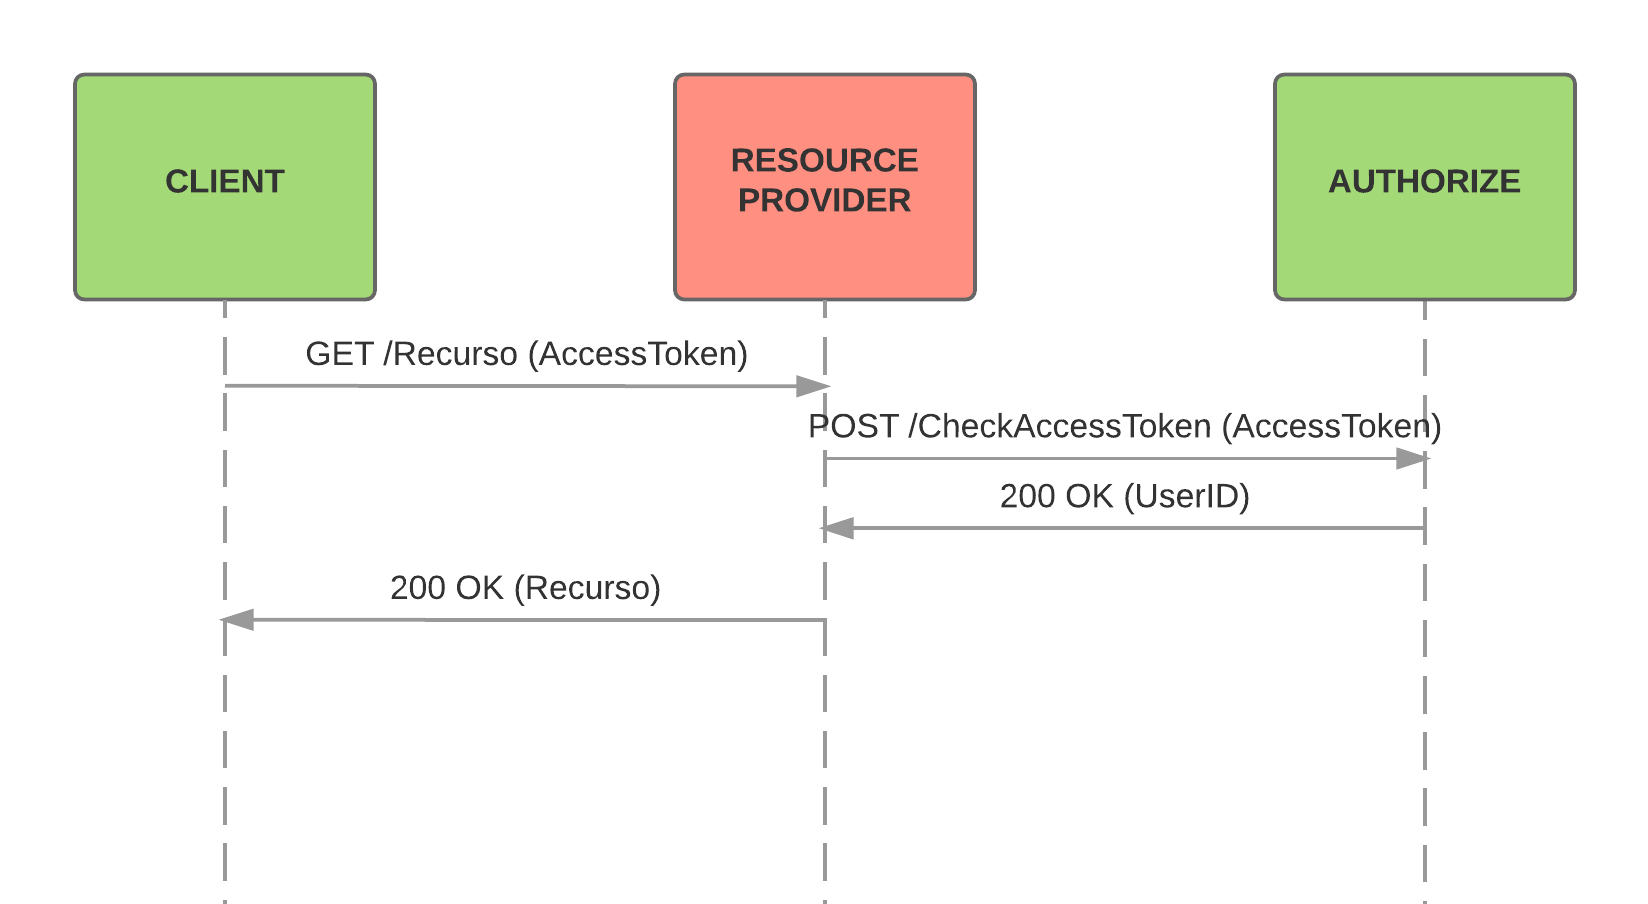
\includegraphics[width=1.1\textwidth]{./images/oauth/diagrama_obtener_recurso.png}
\caption{Diagrama obtener resurso.}
\label{fig:oauth4}
\end{figure}

% #######################   MANUAL DE USO  ##################################

\subsubsection{Manual de Uso}

El uso de este servicio pretende ser intuitivo y facilitar las gestiones de los usuarios, por lo que su uso es muy simple. Seguiremos los siguientes pasos para probar su funcionamiento:

\begin{itemize}
	\item Comprobar que todos los servidores están iniciados.
	
	\item Comprobar que no tenemos ningún firewall bloqueando el acceso.
	
	\item Abrir un navegador web y acceder a la página web de la Notaría \\
		\url{http://XXXX/Seguridad\_NotariaWeb/rest/Index}	\\
		(Figura \ref{fig:oauth5})
	
	\item Pinchar sobre \emph{Formulario de hipoteca}. Nos llevará a la web de identificación.
	
	\item Introducir el DNI/Contraseña y pulsar sobre \emph{Seleccionar archivo} para incluír la imagen de la 		huella digital. Pulsar sobre \emph{Enviar}. \\
	Credenciales válidas:
	\begin{itemize}
		\item DNI: "77777777P" Contraseña: "alumno"
		\item DNI: "23453456L" Contraseña: "alumno"
		\item DNI: "78547854G" Contraseña: "alumno"
	\end{itemize}
	(Figura \ref{fig:oauth6})
\end{itemize}

\begin{figure}[htbp]
\centering
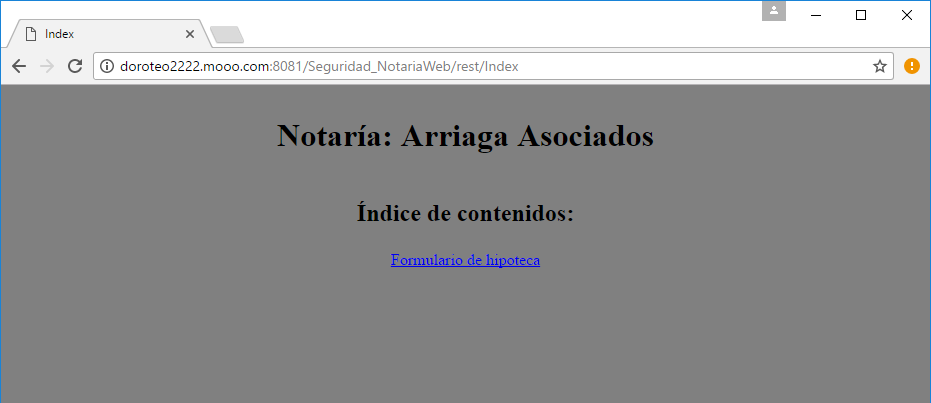
\includegraphics[width=1.1\textwidth]{./images/oauth/notaria_index.png}
\caption{Notaría Index.}
\label{fig:oauth5}
\end{figure}

\begin{figure}[htbp]
\centering
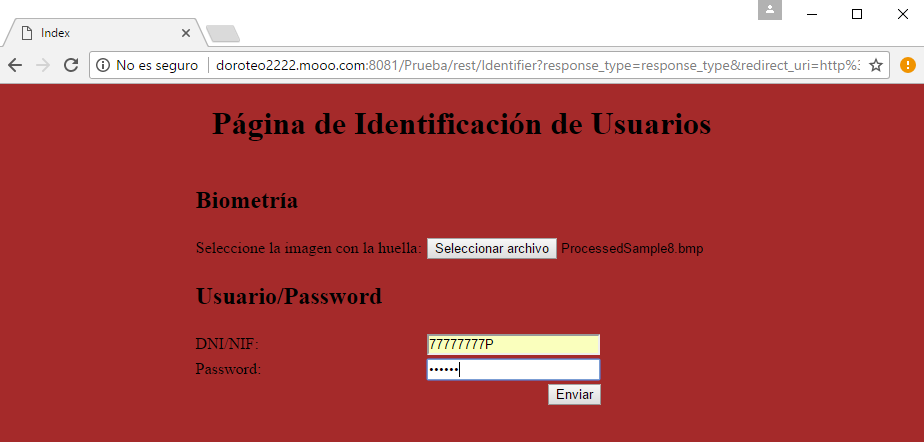
\includegraphics[width=1.1\textwidth]{./images/oauth/IDP_identifier.png}
\caption{IDP identificación.}
\label{fig:oauth6}
\end{figure}

\begin{figure}[htbp]
\centering
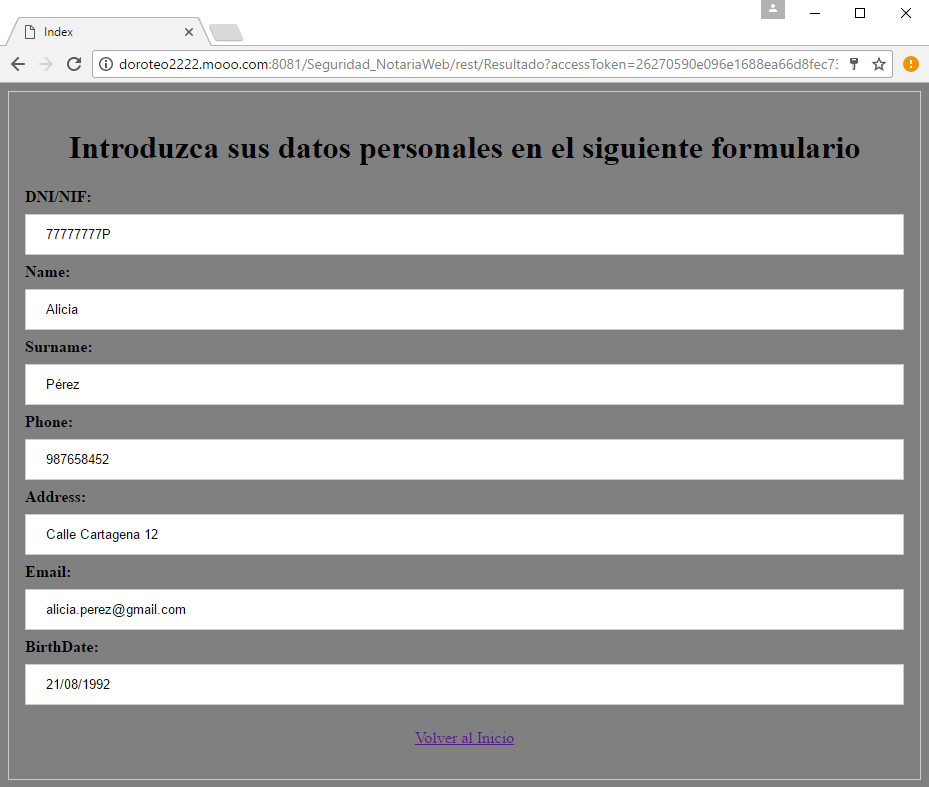
\includegraphics[width=1.1\textwidth]{./images/oauth/form_autocompleted.png}
\caption{Formulario de hipoteca autocompletado.}
\label{fig:oauth7}
\end{figure}


% #######################   NMAP y Metasploit   ##################################

\clearpage
\section{NMAP y Metasploit}
\rhead[\thepage]{\thesection. NMAP y Metasploit}

\subsection{Víctima}
Utilizaremos una máquina virtual de prueba. Esta máquina ha sido creada con vulnerabilidades para la práctica de ataques. La URL de descarga es la \href{wiki.inf.um.es/metasploitable2/metasploitable-linux-2.0.0.zip}{siguiente}. \\

La IP de esta máquina es la \texttt{192.168.62.189}.

\subsection{Atacante}

\subsubsection{NMAP}

El equipo que actuará como atacante hace uso de la herramienta NMAP. Para instalarla ejecutamos el siguiente comando:

\begin{verbatim}
$ sudo apt-get install namp
\end{verbatim}

Establecemos en el archivo \emph{/etc/hosts}, equivalente al DNS local, la IP de la víctima (\texttt{192.168.62.189}) y la denominamos \texttt{metasploitable}, como muestra la figura \ref{fig:nmap1}. \\

\begin{figure}[htbp]
\centering
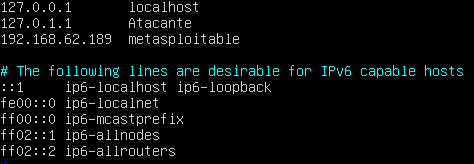
\includegraphics[width=0.5\textwidth]{./images/Atacante_dns_victima.png}
\caption{Atacante\_dns\_victima.}
\label{fig:nmap1}
\end{figure}

De esta forma, tenemos dos opciones para hacer referencia a la víctima. En la figura \ref{fig:nmap2} se observa el resultado de este escaneo simple fruto de cualquiera de estas dos opciones.

\begin{verbatim}
$ nmap 192.168.62.189
$ nmap metasploitable
\end{verbatim}

\begin{figure}[htbp]
\centering
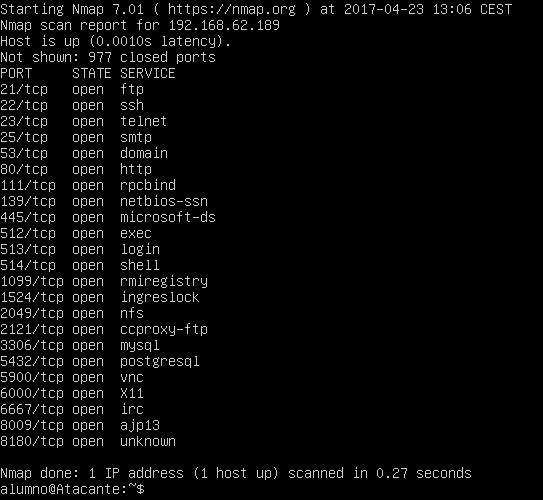
\includegraphics[width=0.8\textwidth]{./images/Atacante_nmap_simplescan.png}
\caption{Atacante\_nmap\_simplescan.}
\label{fig:nmap2}
\end{figure}

De forma un poco más elaborada, se puede ejecutar el escaneo de puertos haciendo uso de otras técnicas:

\begin{itemize}
  \item Mediante listado de equipos: \texttt{\$ nmap 192.168.62.1 192.168.62.10 192.168.62.189}
  \item Mediante subred: \$ nmap 192.168.62.0/24
  \item Mediante un fichero que almacene las IPs (o las expresiones de las mismas) a analizar: \$ nmap -iL hosts.txt, como muestra la figura \ref{fig:nmap3}.
\end{itemize}

\begin{figure}[htbp]
\centering
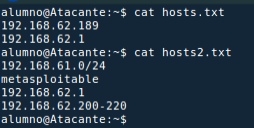
\includegraphics[width=0.4\textwidth]{./images/Atacante_nmapscan_filecomplex.png}
\caption{Atacante\_nmapscan\_filecomplex.}
\label{fig:nmap3}
\end{figure}

\subsubsection{NMAP con Metasploit}

También hemos de instalar Mestasploit para hacer uso de él: \url{https://github.com/rapid7/metasploit-framework/wiki/Nightly-Installers}. Una vez instalado, con \texttt{\$ msfconsole} inicializamos Metasploit y la base de datos asociada. \\

A continuación, realizamos un scanner básico de la red, almacenando el contenido en la base de datos interna y exportándolo completo de la misma a un fichero, para así analizarlo:

\begin{verbatim}
$ db_nmap -v -sV 192.168.62.0/24
$ db_export out_ejercicio1.txt
\end{verbatim}

Como muestra la figura \ref{fig:nmap4}, se observa que en dicho fichero encontramos el contenido del escaneo. Por un lado, podemos ver información del usuario que ha invocado el Metasploit. Seguidamente, tenemos el apartado que refiere a los hosts y servicios que se han encontrado en la dirección de subred que se le ha pasado al escaneo. Por último, podemos observar que el grueso del fichero son los módulos del Metasploit.

\begin{figure}[htbp]
\centering
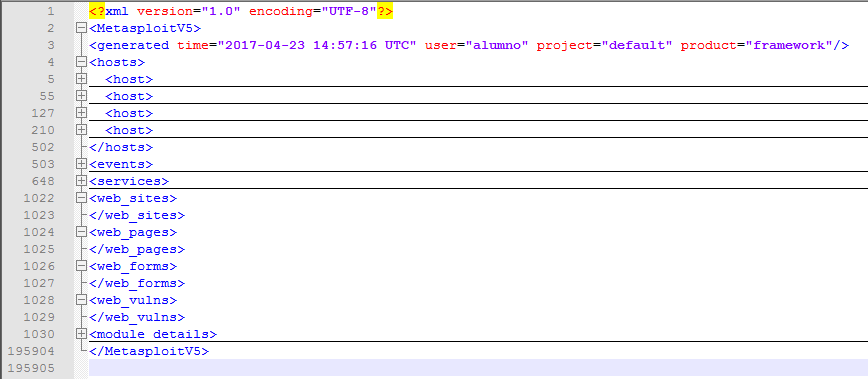
\includegraphics[width=1.0\textwidth]{./images/Atacante_scaner_y_BBDD.png}
\caption{Atacante\_scaner\_y\_BBDD.}
\label{fig:nmap4}
\end{figure}

% #######################   Wireshak: trazas   ##################################

\subsubsection{Wireshak: trazas}

A continuación mostramos algunas trazas obtenidas tras ejecutar ciertos comandos con NMAP.

\begin{itemize}
  \item \texttt{\$ nmap —scan-delay 1000ms -p 20-30 metasploitable}. En el host \texttt{metasploitable} se lanza un escaneo de puertos cada segundo a un puerto diferente entre los puertos 20 al 30, como muestra la figura \ref{fig:nmap5}. El fin principal de realizar un escaneo de puertos de esta forma es evitar ser detectado por la seguridad que pueda tener la subred.

  \begin{figure}[htbp]
  \centering
  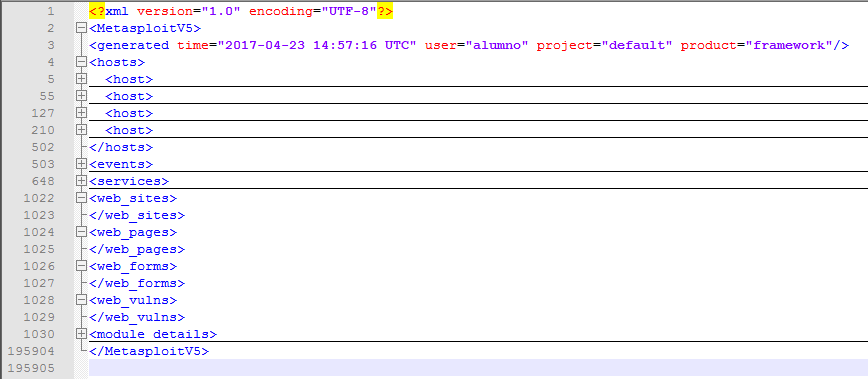
\includegraphics[width=1.0\textwidth]{./images/Atacante_scaner_y_BBDD.png}
  \caption{Atacante\_wireshar\_scaneo\_delay.}
  \label{fig:nmap5}
  \end{figure}

  \item \texttt{\$sudo nmap -sS -mtu 24 -p 80 metasploitable 192.168.62.102}. En el hots \texttt{metasploitable} y en la IP \texttt{192.168.62.102} se lanza un escaneo al puerto 80 con el bit SYN activado, como se muestra en la figura \ref{fig:nmap6} Lo que se hace es enviar un paquete SYN, como si se fuera a abrir una conexión real y después se espera una respuesta. Si se recibe un paquete SYN/ACK esto indica que el puerto está abierto, mientras que si se recibe un RST (reset) indica que no hay nada escuchando en el puerto. Si no se recibe ninguna respuesta después de realizar algunas retransmisiones o se recibe un ICMP entonces el puerto se marca como filtrado.

  \begin{figure}[htbp]
  \centering
  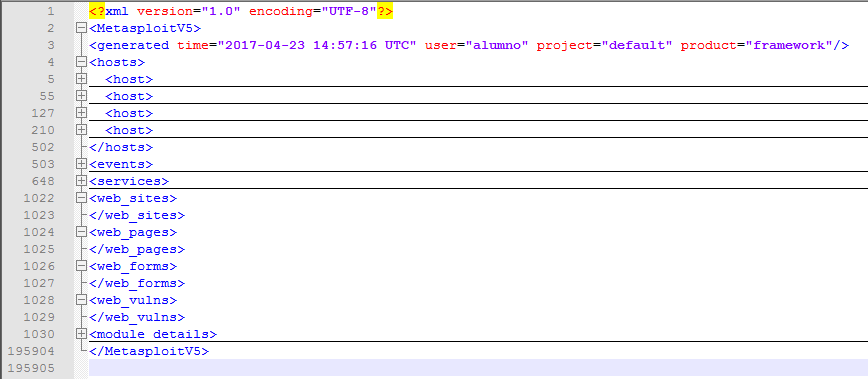
\includegraphics[width=1.0\textwidth]{./images/Atacante_scaner_y_BBDD.png}
  \caption{Atacante\_wireshar\_scaneo\_delay.}
  \label{fig:nmap6}
  \end{figure}
\end{itemize}

% #######################   Scripts NMAP   ##################################

\subsection{Scripts NMAP}
\subsubsection{Scripts /usr/share/nmap/scripts}
En la instalación de NMAP se crea el directorio \textit{/usr/share/nmap/scripts}, este directorio contiene una lista de scripts implementados por otros usuarios y que están diseñados para ser invocados desde el comando nmap. A continuación se describen algunos:
\begin{itemize}
\item \texttt{http-git.nse}: Realiza una conexión al puerto 80 de la víctima en busca de un servidor web activo, si el puerto está abierto, se intenta localizar un directorio \emph{.git}. La existencia de este directorio implica que la víctima está realizando un control de versiones, por tanto, el siguiente paso que realiza el script es la búsqueda de coincidencias en \emph{Github}, si se encuentran coincidencias (por un perfil o proyecto público), se muestran un mensaje al usuario con toda la información que se ha podido extraer de la víctima de su repositorio.
\item \texttt{smb-server-stats.nse}: Este script explota una un fallo de \emph{Samba} corriendo sobre sistemas operativos de Windows, este vulnerabilidad permite que un usuario externo pueda solicitar los datos estadísticos del servicio, recopilando así valiosa información de los archivos que se comparten.
\item \texttt{ssh2-enum-algos.nse}: Devuelve los algoritmos de cifrado y compresión que tiene implementados la víctima. Esta información puede ser muy útil para reducir considerablemente el tiempo de los ataques por fuerza bruta.
\item \texttt{dhcp-discover.nse}: Script que recopila información del servidor DHCP de la red, se imprimirá por pantalla al usuario el valor de cada uno de los campos que se obtienen del DHCP (Gateway, mácara de subred, router, nombre de dominio, etc...). Para el funcionamiento del script no es necesario consumir una dirección IP.
\end{itemize}
\subsubsection{Realización de script básico}
Se pueden crear nuevos scripts adaptados a nuestras necesidades, que automaticen tareas habituales, o repetitivas. En la siguiente url \url{http://nmap.org/book/nse-tutorial.html} se describe la estructura que debe tener el script. Para poner en práctica este apartado, a continuación, incluye el contenido de un script realizado por nosotros, las acciones que realiza son las siguientes:
\begin{itemize}
\item Comprobar si el equipo objeto tiene el puerto 80 abierto (el número de puerto se puede cambiar a la hora de ejecutar el comando)
\item En el caso de que se cumpla el paso anterior, se entiende que existe un servidor web en el equipo, por tanto, se solicita la página \textit{index.html}, dicha página se crea por defecto en los navegadores web.
\item La página web descargada se almacena en un fichero con el mismo nombre \textit{index.html}
\end{itemize}
Para ejecutar el script, se debe escribir el siguiente comando:
\begin{verbatim}
	$ nmap -p 80 <ip> --script=http-index
\end{verbatim}
\lstinputlisting[breaklines]{doc/http-index.nse}
El script contiene un control de errores, por lo que se mostrará uno de los siguientes resultados:
\begin{itemize}
	\item ''ERROR: Fallo al obtener la url index.html"
	\item ''ERROR: Fallo al crear/abrir el fichero index.html"
	\item ''index.html Obtenido correctamente!"
\end{itemize}

% #######################   COMANDO PORTSCAN   ##################################

\subsubsection{Comando Portscan}
Accedemos a la consola de Metasploit con el comando \emph{\$msfconsole}, para encontrar las modalidades existentes de Portscan, lanzamos la búsqueda con \emph{\$search portscan}, el resultado se puede ver en la figura \ref{fig:meta2}.

\begin{figure}[htbp]
\centering
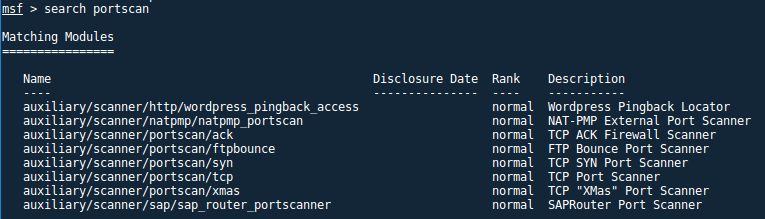
\includegraphics[width=1.0\textwidth]{./images/Atacante_metasploit_portscan_search.png}
\caption{Metasploit Portscan Search}
\label{fig:meta2}
\end{figure}

\begin{enumerate}
\item Para este ejemplo haremos uso de \emph{auxiliary/scanner/portscan/tcp}, para ello, lo seleccionamos ejecutando \emph{\$use auxiliary/scanner/portscan/tcp}.
\item Visualizamos los diferentes parámetros de configuración que permite con el comando \emph{\$show options}.
\item Ajustamos el número de hilos y la ip de la víctima.
\item Lanzamos el escaneo con el comando \emph{\$run}. Se muestra el resultado de la ejecución en la imagen \ref{fig:meta1}.
\item El funcionamiento del comando \emph{portscan} es muy similar al de Nmap, con la ventaja de poder ajustar el número de hilos que queremos dedicar al escaneo.
\end{enumerate}

\begin{figure}[htbp]
\centering
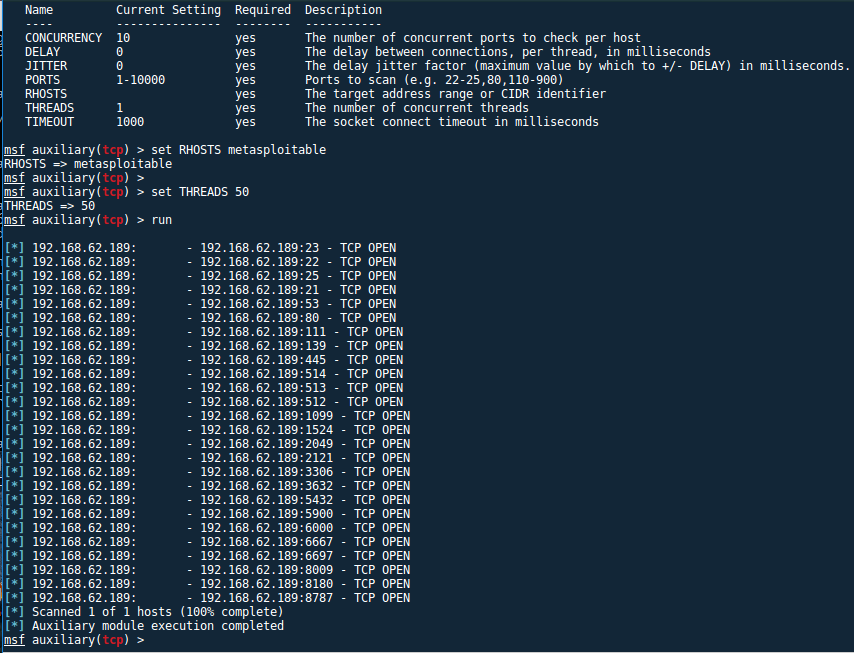
\includegraphics[width=1.0\textwidth]{./images/Atacante_metasploit_portscan.png}
\caption{Metasploit Portscan}
\label{fig:meta1}
\end{figure}

% #######################   EXPLOTAR VULNERABILIDADES   ##################################

\clearpage
\section{Explotar Vulnerabilidades}
\rhead[\thepage]{\thesection. Explotar Vulnerabilidades}

Para usuarios que no son expertos en el uso de Metasploit, se recomienda el uso de la interfaz gráfica del programa, que se puede descargar desde el \href{https://www.rapid7.com/products/metasploit/download/}{siguiente enlace}. La instalación es muy simple en Linux, basta con descargarse el programa, convertirlo en ejecutable (\texttt{\$ chmod 777 metasploit-latest-linux-x64-installer.run}) y ejecutar el fichero (\texttt{.run}). Se abrirá un instalador gráfico intuitivo. \\

Para hacer uso del programa, abrimos un navegador web y accedemos a la URL que se nos indicó durante la instalación, si no hemos modificado las opciones por defecto, será \emph{https://localhost:3790/}. En la figura \ref{fig:meta3} podemos ver la apariencia.

\begin{figure}[htbp]
\centering
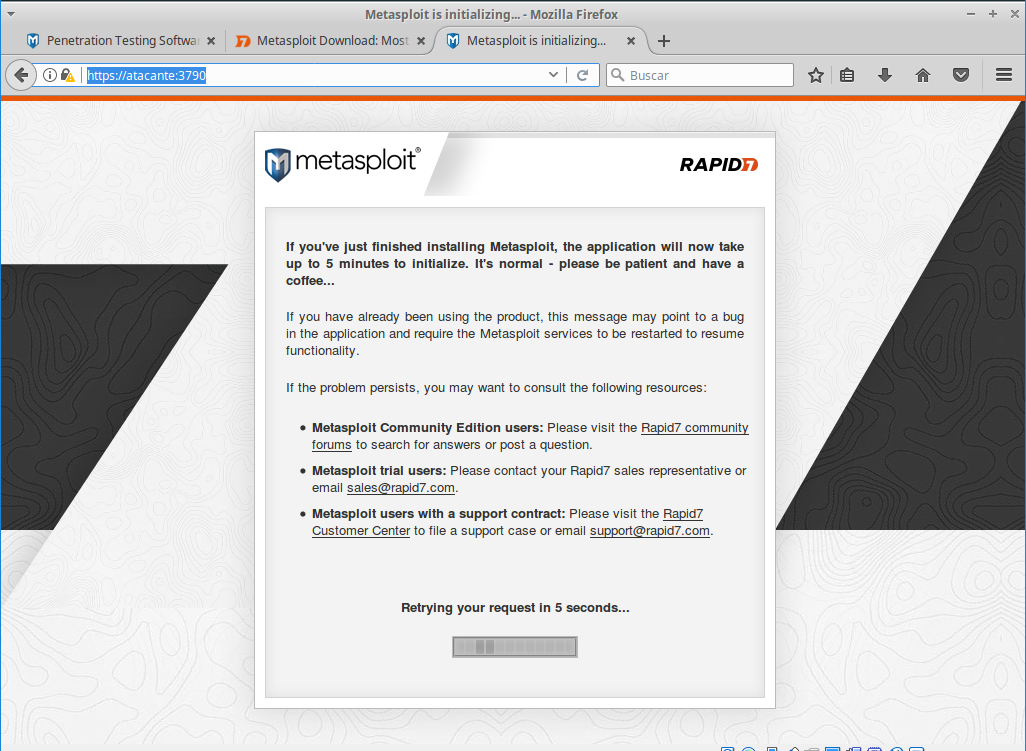
\includegraphics[width=1.0\textwidth]{./images/Atacante_metasploit_grafico.png}
\caption{Metasploit Gráfico}
\label{fig:meta3}
\end{figure}

\end{document}
